% Created by tikzDevice version 0.10.1 on 2017-10-30 17:28:41
% !TEX encoding = UTF-8 Unicode
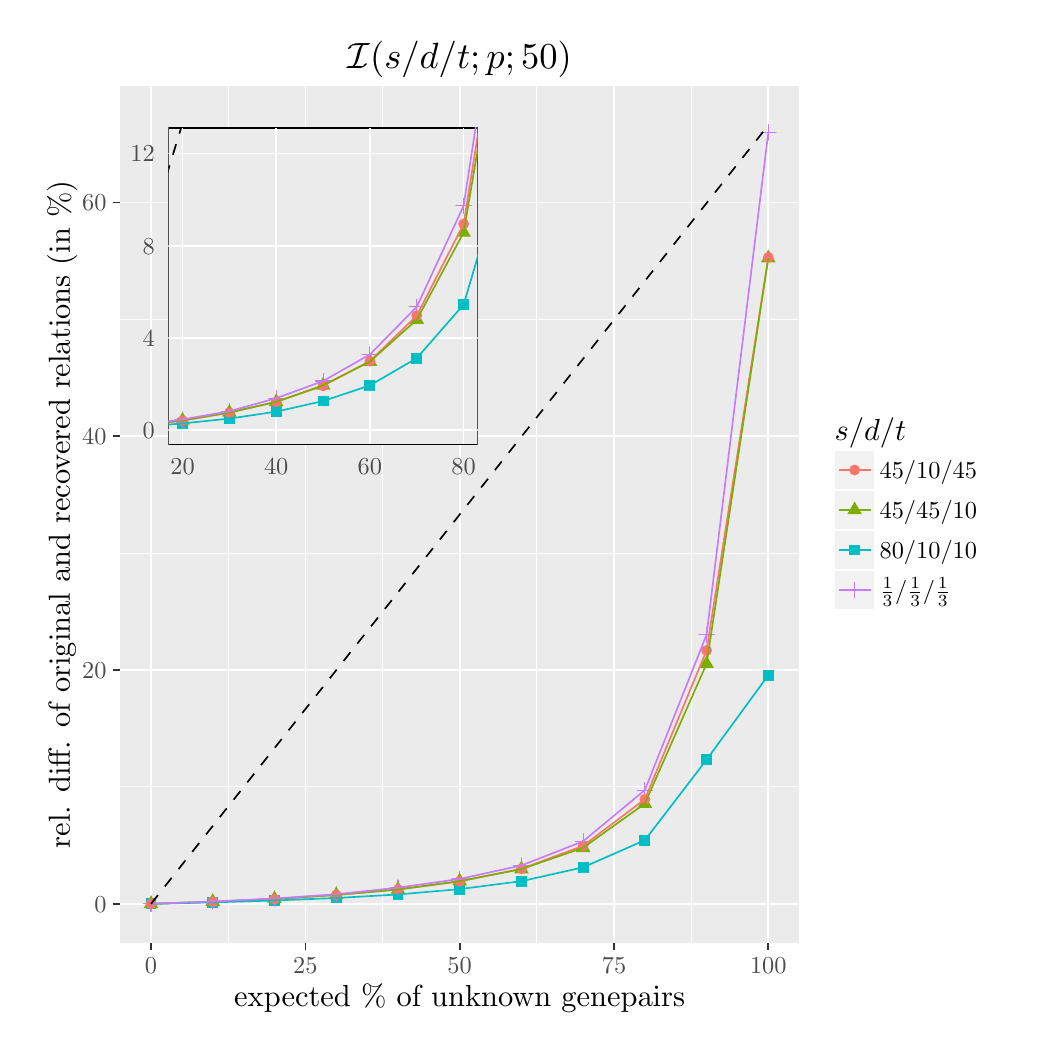
\begin{tikzpicture}[x=1pt,y=1pt]
\definecolor{fillColor}{RGB}{255,255,255}
\path[use as bounding box,fill=fillColor,fill opacity=0.00] (0,0) rectangle (361.35,361.35);
\begin{scope}
\path[clip] (  0.00,  0.00) rectangle (361.35,361.35);
\definecolor{drawColor}{RGB}{255,255,255}
\definecolor{fillColor}{RGB}{255,255,255}

\path[draw=drawColor,line width= 0.6pt,line join=round,line cap=round,fill=fillColor] (  0.00,  0.00) rectangle (361.35,361.35);
\end{scope}
\begin{scope}
\path[clip] ( 33.42, 30.69) rectangle (278.78,340.16);
\definecolor{fillColor}{gray}{0.92}

\path[fill=fillColor] ( 33.42, 30.69) rectangle (278.78,340.16);
\definecolor{drawColor}{RGB}{255,255,255}

\path[draw=drawColor,line width= 0.3pt,line join=round] ( 33.42, 87.00) --
	(278.78, 87.00);

\path[draw=drawColor,line width= 0.3pt,line join=round] ( 33.42,171.48) --
	(278.78,171.48);

\path[draw=drawColor,line width= 0.3pt,line join=round] ( 33.42,255.97) --
	(278.78,255.97);

\path[draw=drawColor,line width= 0.3pt,line join=round] ( 72.46, 30.69) --
	( 72.46,340.16);

\path[draw=drawColor,line width= 0.3pt,line join=round] (128.22, 30.69) --
	(128.22,340.16);

\path[draw=drawColor,line width= 0.3pt,line join=round] (183.98, 30.69) --
	(183.98,340.16);

\path[draw=drawColor,line width= 0.3pt,line join=round] (239.75, 30.69) --
	(239.75,340.16);

\path[draw=drawColor,line width= 0.6pt,line join=round] ( 33.42, 44.75) --
	(278.78, 44.75);

\path[draw=drawColor,line width= 0.6pt,line join=round] ( 33.42,129.24) --
	(278.78,129.24);

\path[draw=drawColor,line width= 0.6pt,line join=round] ( 33.42,213.73) --
	(278.78,213.73);

\path[draw=drawColor,line width= 0.6pt,line join=round] ( 33.42,298.21) --
	(278.78,298.21);

\path[draw=drawColor,line width= 0.6pt,line join=round] ( 44.58, 30.69) --
	( 44.58,340.16);

\path[draw=drawColor,line width= 0.6pt,line join=round] (100.34, 30.69) --
	(100.34,340.16);

\path[draw=drawColor,line width= 0.6pt,line join=round] (156.10, 30.69) --
	(156.10,340.16);

\path[draw=drawColor,line width= 0.6pt,line join=round] (211.87, 30.69) --
	(211.87,340.16);

\path[draw=drawColor,line width= 0.6pt,line join=round] (267.63, 30.69) --
	(267.63,340.16);
\definecolor{fillColor}{RGB}{0,191,196}

\path[fill=fillColor] ( 42.61, 42.79) --
	( 46.54, 42.79) --
	( 46.54, 46.72) --
	( 42.61, 46.72) --
	cycle;

\path[fill=fillColor] ( 64.92, 43.31) --
	( 68.84, 43.31) --
	( 68.84, 47.23) --
	( 64.92, 47.23) --
	cycle;

\path[fill=fillColor] ( 87.22, 44.00) --
	( 91.15, 44.00) --
	( 91.15, 47.93) --
	( 87.22, 47.93) --
	cycle;

\path[fill=fillColor] (109.53, 44.89) --
	(113.45, 44.89) --
	(113.45, 48.81) --
	(109.53, 48.81) --
	cycle;

\path[fill=fillColor] (131.84, 46.17) --
	(135.76, 46.17) --
	(135.76, 50.09) --
	(131.84, 50.09) --
	cycle;

\path[fill=fillColor] (154.14, 48.11) --
	(158.06, 48.11) --
	(158.06, 52.03) --
	(154.14, 52.03) --
	cycle;

\path[fill=fillColor] (176.45, 50.98) --
	(180.37, 50.98) --
	(180.37, 54.90) --
	(176.45, 54.90) --
	cycle;

\path[fill=fillColor] (198.75, 55.97) --
	(202.68, 55.97) --
	(202.68, 59.90) --
	(198.75, 59.90) --
	cycle;

\path[fill=fillColor] (221.06, 65.79) --
	(224.98, 65.79) --
	(224.98, 69.72) --
	(221.06, 69.72) --
	cycle;

\path[fill=fillColor] (243.36, 94.87) --
	(247.29, 94.87) --
	(247.29, 98.80) --
	(243.36, 98.80) --
	cycle;

\path[fill=fillColor] (265.67,125.41) --
	(269.59,125.41) --
	(269.59,129.33) --
	(265.67,129.33) --
	cycle;
\definecolor{drawColor}{RGB}{199,124,255}

\path[draw=drawColor,line width= 0.4pt,line join=round,line cap=round] ( 41.80, 44.75) -- ( 47.35, 44.75);

\path[draw=drawColor,line width= 0.4pt,line join=round,line cap=round] ( 44.58, 41.98) -- ( 44.58, 47.53);

\path[draw=drawColor,line width= 0.4pt,line join=round,line cap=round] ( 64.11, 45.59) -- ( 69.66, 45.59);

\path[draw=drawColor,line width= 0.4pt,line join=round,line cap=round] ( 66.88, 42.81) -- ( 66.88, 48.36);

\path[draw=drawColor,line width= 0.4pt,line join=round,line cap=round] ( 86.41, 46.69) -- ( 91.96, 46.69);

\path[draw=drawColor,line width= 0.4pt,line join=round,line cap=round] ( 89.19, 43.92) -- ( 89.19, 49.47);

\path[draw=drawColor,line width= 0.4pt,line join=round,line cap=round] (108.72, 48.21) -- (114.27, 48.21);

\path[draw=drawColor,line width= 0.4pt,line join=round,line cap=round] (111.49, 45.43) -- (111.49, 50.98);

\path[draw=drawColor,line width= 0.4pt,line join=round,line cap=round] (131.02, 50.59) -- (136.57, 50.59);

\path[draw=drawColor,line width= 0.4pt,line join=round,line cap=round] (133.80, 47.81) -- (133.80, 53.36);

\path[draw=drawColor,line width= 0.4pt,line join=round,line cap=round] (153.33, 53.74) -- (158.88, 53.74);

\path[draw=drawColor,line width= 0.4pt,line join=round,line cap=round] (156.10, 50.96) -- (156.10, 56.51);

\path[draw=drawColor,line width= 0.4pt,line join=round,line cap=round] (175.63, 58.61) -- (181.18, 58.61);

\path[draw=drawColor,line width= 0.4pt,line join=round,line cap=round] (178.41, 55.84) -- (178.41, 61.39);

\path[draw=drawColor,line width= 0.4pt,line join=round,line cap=round] (197.94, 67.35) -- (203.49, 67.35);

\path[draw=drawColor,line width= 0.4pt,line join=round,line cap=round] (200.71, 64.57) -- (200.71, 70.12);

\path[draw=drawColor,line width= 0.4pt,line join=round,line cap=round] (220.24, 85.86) -- (225.79, 85.86);

\path[draw=drawColor,line width= 0.4pt,line join=round,line cap=round] (223.02, 83.08) -- (223.02, 88.63);

\path[draw=drawColor,line width= 0.4pt,line join=round,line cap=round] (242.55,141.99) -- (248.10,141.99);

\path[draw=drawColor,line width= 0.4pt,line join=round,line cap=round] (245.32,139.22) -- (245.32,144.77);

\path[draw=drawColor,line width= 0.4pt,line join=round,line cap=round] (264.85,323.52) -- (270.40,323.52);

\path[draw=drawColor,line width= 0.4pt,line join=round,line cap=round] (267.63,320.75) -- (267.63,326.30);
\definecolor{fillColor}{RGB}{124,174,0}

\path[fill=fillColor] ( 44.58, 47.80) --
	( 47.22, 43.23) --
	( 41.93, 43.23) --
	cycle;

\path[fill=fillColor] ( 66.88, 48.58) --
	( 69.52, 44.00) --
	( 64.24, 44.00) --
	cycle;

\path[fill=fillColor] ( 89.19, 49.57) --
	( 91.83, 44.99) --
	( 86.54, 44.99) --
	cycle;

\path[fill=fillColor] (111.49, 51.03) --
	(114.13, 46.46) --
	(108.85, 46.46) --
	cycle;

\path[fill=fillColor] (133.80, 52.98) --
	(136.44, 48.40) --
	(131.15, 48.40) --
	cycle;

\path[fill=fillColor] (156.10, 56.01) --
	(158.75, 51.43) --
	(153.46, 51.43) --
	cycle;

\path[fill=fillColor] (178.41, 60.35) --
	(181.05, 55.77) --
	(175.77, 55.77) --
	cycle;

\path[fill=fillColor] (200.71, 68.04) --
	(203.36, 63.46) --
	(198.07, 63.46) --
	cycle;

\path[fill=fillColor] (223.02, 84.03) --
	(225.66, 79.45) --
	(220.38, 79.45) --
	cycle;

\path[fill=fillColor] (245.32,134.55) --
	(247.97,129.97) --
	(242.68,129.97) --
	cycle;

\path[fill=fillColor] (267.63,281.16) --
	(270.27,276.58) --
	(264.99,276.58) --
	cycle;
\definecolor{fillColor}{RGB}{248,118,109}

\path[fill=fillColor] ( 44.58, 44.75) circle (  1.96);

\path[fill=fillColor] ( 66.88, 45.49) circle (  1.96);

\path[fill=fillColor] ( 89.19, 46.46) circle (  1.96);

\path[fill=fillColor] (111.49, 47.94) circle (  1.96);

\path[fill=fillColor] (133.80, 49.91) circle (  1.96);

\path[fill=fillColor] (156.10, 52.86) circle (  1.96);

\path[fill=fillColor] (178.41, 57.39) circle (  1.96);

\path[fill=fillColor] (200.71, 65.73) circle (  1.96);

\path[fill=fillColor] (223.02, 82.53) circle (  1.96);

\path[fill=fillColor] (245.32,136.32) circle (  1.96);

\path[fill=fillColor] (267.63,278.34) circle (  1.96);
\definecolor{drawColor}{RGB}{248,118,109}

\path[draw=drawColor,line width= 0.6pt,line join=round] ( 44.58, 44.75) --
	( 66.88, 45.49) --
	( 89.19, 46.46) --
	(111.49, 47.94) --
	(133.80, 49.91) --
	(156.10, 52.86) --
	(178.41, 57.39) --
	(200.71, 65.73) --
	(223.02, 82.53) --
	(245.32,136.32) --
	(267.63,278.34);
\definecolor{drawColor}{RGB}{124,174,0}

\path[draw=drawColor,line width= 0.6pt,line join=round] ( 44.58, 44.75) --
	( 66.88, 45.52) --
	( 89.19, 46.52) --
	(111.49, 47.98) --
	(133.80, 49.93) --
	(156.10, 52.96) --
	(178.41, 57.30) --
	(200.71, 64.99) --
	(223.02, 80.98) --
	(245.32,131.50) --
	(267.63,278.11);
\definecolor{drawColor}{RGB}{0,191,196}

\path[draw=drawColor,line width= 0.6pt,line join=round] ( 44.58, 44.75) --
	( 66.88, 45.27) --
	( 89.19, 45.96) --
	(111.49, 46.85) --
	(133.80, 48.13) --
	(156.10, 50.07) --
	(178.41, 52.94) --
	(200.71, 57.93) --
	(223.02, 67.75) --
	(245.32, 96.83) --
	(267.63,127.37);
\definecolor{drawColor}{RGB}{199,124,255}

\path[draw=drawColor,line width= 0.6pt,line join=round] ( 44.58, 44.75) --
	( 66.88, 45.59) --
	( 89.19, 46.69) --
	(111.49, 48.21) --
	(133.80, 50.59) --
	(156.10, 53.74) --
	(178.41, 58.61) --
	(200.71, 67.35) --
	(223.02, 85.86) --
	(245.32,141.99) --
	(267.63,323.52);
\definecolor{drawColor}{RGB}{0,0,0}

\path[draw=drawColor,line width= 0.6pt,dash pattern=on 4pt off 4pt ,line join=round] ( 44.58, 44.75) --
	( 55.73, 58.82) --
	( 66.88, 72.89) --
	( 78.03, 86.95) --
	( 89.19,101.02) --
	(100.34,115.09) --
	(111.49,129.16) --
	(122.64,143.22) --
	(133.80,157.29) --
	(144.95,171.36) --
	(156.10,185.42) --
	(167.26,199.49) --
	(178.41,213.56) --
	(189.56,227.62) --
	(200.71,241.69) --
	(211.87,255.76) --
	(223.02,269.82) --
	(234.17,283.89) --
	(245.32,297.96) --
	(256.48,312.03) --
	(267.63,326.09);
\end{scope}
\begin{scope}
\path[clip] (  0.00,  0.00) rectangle (361.35,361.35);
\definecolor{drawColor}{gray}{0.30}

\node[text=drawColor,anchor=base east,inner sep=0pt, outer sep=0pt, scale=  0.88] at ( 28.47, 41.72) {0};

\node[text=drawColor,anchor=base east,inner sep=0pt, outer sep=0pt, scale=  0.88] at ( 28.47,126.21) {20};

\node[text=drawColor,anchor=base east,inner sep=0pt, outer sep=0pt, scale=  0.88] at ( 28.47,210.70) {40};

\node[text=drawColor,anchor=base east,inner sep=0pt, outer sep=0pt, scale=  0.88] at ( 28.47,295.18) {60};
\end{scope}
\begin{scope}
\path[clip] (  0.00,  0.00) rectangle (361.35,361.35);
\definecolor{drawColor}{gray}{0.20}

\path[draw=drawColor,line width= 0.6pt,line join=round] ( 30.67, 44.75) --
	( 33.42, 44.75);

\path[draw=drawColor,line width= 0.6pt,line join=round] ( 30.67,129.24) --
	( 33.42,129.24);

\path[draw=drawColor,line width= 0.6pt,line join=round] ( 30.67,213.73) --
	( 33.42,213.73);

\path[draw=drawColor,line width= 0.6pt,line join=round] ( 30.67,298.21) --
	( 33.42,298.21);
\end{scope}
\begin{scope}
\path[clip] (  0.00,  0.00) rectangle (361.35,361.35);
\definecolor{drawColor}{gray}{0.20}

\path[draw=drawColor,line width= 0.6pt,line join=round] ( 44.58, 27.94) --
	( 44.58, 30.69);

\path[draw=drawColor,line width= 0.6pt,line join=round] (100.34, 27.94) --
	(100.34, 30.69);

\path[draw=drawColor,line width= 0.6pt,line join=round] (156.10, 27.94) --
	(156.10, 30.69);

\path[draw=drawColor,line width= 0.6pt,line join=round] (211.87, 27.94) --
	(211.87, 30.69);

\path[draw=drawColor,line width= 0.6pt,line join=round] (267.63, 27.94) --
	(267.63, 30.69);
\end{scope}
\begin{scope}
\path[clip] (  0.00,  0.00) rectangle (361.35,361.35);
\definecolor{drawColor}{gray}{0.30}

\node[text=drawColor,anchor=base,inner sep=0pt, outer sep=0pt, scale=  0.88] at ( 44.58, 19.68) {0};

\node[text=drawColor,anchor=base,inner sep=0pt, outer sep=0pt, scale=  0.88] at (100.34, 19.68) {25};

\node[text=drawColor,anchor=base,inner sep=0pt, outer sep=0pt, scale=  0.88] at (156.10, 19.68) {50};

\node[text=drawColor,anchor=base,inner sep=0pt, outer sep=0pt, scale=  0.88] at (211.87, 19.68) {75};

\node[text=drawColor,anchor=base,inner sep=0pt, outer sep=0pt, scale=  0.88] at (267.63, 19.68) {100};
\end{scope}
\begin{scope}
\path[clip] (  0.00,  0.00) rectangle (361.35,361.35);
\definecolor{drawColor}{RGB}{0,0,0}

\node[text=drawColor,anchor=base,inner sep=0pt, outer sep=0pt, scale=  1.10] at (156.10,  7.70) {expected \% of unknown genepairs};
\end{scope}
\begin{scope}
\path[clip] (  0.00,  0.00) rectangle (361.35,361.35);
\definecolor{drawColor}{RGB}{0,0,0}

\node[text=drawColor,rotate= 90.00,anchor=base,inner sep=0pt, outer sep=0pt, scale=  1.10] at ( 15.28,185.42) {rel. diff. of original and recovered relations (in \%)};
\end{scope}
\begin{scope}
\path[clip] (  0.00,  0.00) rectangle (361.35,361.35);
\definecolor{fillColor}{RGB}{255,255,255}

\path[fill=fillColor] (287.32,146.65) rectangle (347.31,224.19);
\end{scope}
\begin{scope}
\path[clip] (  0.00,  0.00) rectangle (361.35,361.35);
\definecolor{drawColor}{RGB}{0,0,0}

\node[text=drawColor,anchor=base west,inner sep=0pt, outer sep=0pt, scale=  1.10] at (291.59,212.35) {$\mathfrak{s}/\mathfrak{d}/\mathfrak{t}$};
\end{scope}
\begin{scope}
\path[clip] (  0.00,  0.00) rectangle (361.35,361.35);
\definecolor{drawColor}{RGB}{255,255,255}
\definecolor{fillColor}{gray}{0.95}

\path[draw=drawColor,line width= 0.6pt,line join=round,line cap=round,fill=fillColor] (291.59,194.28) rectangle (306.04,208.74);
\end{scope}
\begin{scope}
\path[clip] (  0.00,  0.00) rectangle (361.35,361.35);
\definecolor{fillColor}{RGB}{248,118,109}

\path[fill=fillColor] (298.81,201.51) circle (  1.96);
\end{scope}
\begin{scope}
\path[clip] (  0.00,  0.00) rectangle (361.35,361.35);
\definecolor{drawColor}{RGB}{248,118,109}

\path[draw=drawColor,line width= 0.6pt,line join=round] (293.03,201.51) -- (304.59,201.51);
\end{scope}
\begin{scope}
\path[clip] (  0.00,  0.00) rectangle (361.35,361.35);
\definecolor{drawColor}{RGB}{255,255,255}
\definecolor{fillColor}{gray}{0.95}

\path[draw=drawColor,line width= 0.6pt,line join=round,line cap=round,fill=fillColor] (291.59,179.83) rectangle (306.04,194.28);
\end{scope}
\begin{scope}
\path[clip] (  0.00,  0.00) rectangle (361.35,361.35);
\definecolor{fillColor}{RGB}{124,174,0}

\path[fill=fillColor] (298.81,190.11) --
	(301.45,185.53) --
	(296.17,185.53) --
	cycle;
\end{scope}
\begin{scope}
\path[clip] (  0.00,  0.00) rectangle (361.35,361.35);
\definecolor{drawColor}{RGB}{124,174,0}

\path[draw=drawColor,line width= 0.6pt,line join=round] (293.03,187.06) -- (304.59,187.06);
\end{scope}
\begin{scope}
\path[clip] (  0.00,  0.00) rectangle (361.35,361.35);
\definecolor{drawColor}{RGB}{255,255,255}
\definecolor{fillColor}{gray}{0.95}

\path[draw=drawColor,line width= 0.6pt,line join=round,line cap=round,fill=fillColor] (291.59,165.37) rectangle (306.04,179.83);
\end{scope}
\begin{scope}
\path[clip] (  0.00,  0.00) rectangle (361.35,361.35);
\definecolor{fillColor}{RGB}{0,191,196}

\path[fill=fillColor] (296.85,170.64) --
	(300.77,170.64) --
	(300.77,174.56) --
	(296.85,174.56) --
	cycle;
\end{scope}
\begin{scope}
\path[clip] (  0.00,  0.00) rectangle (361.35,361.35);
\definecolor{drawColor}{RGB}{0,191,196}

\path[draw=drawColor,line width= 0.6pt,line join=round] (293.03,172.60) -- (304.59,172.60);
\end{scope}
\begin{scope}
\path[clip] (  0.00,  0.00) rectangle (361.35,361.35);
\definecolor{drawColor}{RGB}{255,255,255}
\definecolor{fillColor}{gray}{0.95}

\path[draw=drawColor,line width= 0.6pt,line join=round,line cap=round,fill=fillColor] (291.59,150.92) rectangle (306.04,165.37);
\end{scope}
\begin{scope}
\path[clip] (  0.00,  0.00) rectangle (361.35,361.35);
\definecolor{drawColor}{RGB}{199,124,255}

\path[draw=drawColor,line width= 0.4pt,line join=round,line cap=round] (296.04,158.15) -- (301.59,158.15);

\path[draw=drawColor,line width= 0.4pt,line join=round,line cap=round] (298.81,155.37) -- (298.81,160.92);
\end{scope}
\begin{scope}
\path[clip] (  0.00,  0.00) rectangle (361.35,361.35);
\definecolor{drawColor}{RGB}{199,124,255}

\path[draw=drawColor,line width= 0.6pt,line join=round] (293.03,158.15) -- (304.59,158.15);
\end{scope}
\begin{scope}
\path[clip] (  0.00,  0.00) rectangle (361.35,361.35);
\definecolor{drawColor}{RGB}{0,0,0}

\node[text=drawColor,anchor=base west,inner sep=0pt, outer sep=0pt, scale=  0.88] at (307.85,198.48) {$45/10/45$};
\end{scope}
\begin{scope}
\path[clip] (  0.00,  0.00) rectangle (361.35,361.35);
\definecolor{drawColor}{RGB}{0,0,0}

\node[text=drawColor,anchor=base west,inner sep=0pt, outer sep=0pt, scale=  0.88] at (307.85,184.02) {$45/45/10$};
\end{scope}
\begin{scope}
\path[clip] (  0.00,  0.00) rectangle (361.35,361.35);
\definecolor{drawColor}{RGB}{0,0,0}

\node[text=drawColor,anchor=base west,inner sep=0pt, outer sep=0pt, scale=  0.88] at (307.85,169.57) {$80/10/10$};
\end{scope}
\begin{scope}
\path[clip] (  0.00,  0.00) rectangle (361.35,361.35);
\definecolor{drawColor}{RGB}{0,0,0}

\node[text=drawColor,anchor=base west,inner sep=0pt, outer sep=0pt, scale=  0.88] at (307.85,155.12) {$\frac{1}{3}/\frac{1}{3}/\frac{1}{3}$};
\end{scope}
\begin{scope}
\path[clip] (  0.00,  0.00) rectangle (361.35,361.35);
\definecolor{drawColor}{RGB}{0,0,0}

\node[text=drawColor,anchor=base,inner sep=0pt, outer sep=0pt, scale=  1.32] at (156.10,346.76) {$\mathcal{I}(\mathfrak{s}/\mathfrak{d}/\mathfrak{t};p;50)$};
\end{scope}
\begin{scope}
\path[clip] ( 54.20,216.81) rectangle (162.61,325.21);
\definecolor{drawColor}{RGB}{255,255,255}
\definecolor{fillColor}{RGB}{255,255,255}

\path[draw=drawColor,line width= 0.6pt,line join=round,line cap=round,fill=fillColor] ( 54.20,216.81) rectangle (162.61,325.21);
\end{scope}
\begin{scope}
\path[clip] ( 50.88,210.75) rectangle (162.61,325.21);
\definecolor{drawColor}{RGB}{0,0,0}
\definecolor{fillColor}{gray}{0.92}

\path[draw=drawColor,line width= 0.6pt,line join=round,line cap=round,fill=fillColor] ( 50.88,210.75) rectangle (162.61,325.21);
\definecolor{drawColor}{RGB}{255,255,255}

\path[draw=drawColor,line width= 0.6pt,line join=round] ( 50.88,215.95) --
	(162.61,215.95);

\path[draw=drawColor,line width= 0.6pt,line join=round] ( 50.88,249.25) --
	(162.61,249.25);

\path[draw=drawColor,line width= 0.6pt,line join=round] ( 50.88,282.55) --
	(162.61,282.55);

\path[draw=drawColor,line width= 0.6pt,line join=round] ( 50.88,315.85) --
	(162.61,315.85);

\path[draw=drawColor,line width= 0.6pt,line join=round] ( 55.96,210.75) --
	( 55.96,325.21);

\path[draw=drawColor,line width= 0.6pt,line join=round] ( 89.81,210.75) --
	( 89.81,325.21);

\path[draw=drawColor,line width= 0.6pt,line join=round] (123.67,210.75) --
	(123.67,325.21);

\path[draw=drawColor,line width= 0.6pt,line join=round] (157.53,210.75) --
	(157.53,325.21);
\definecolor{fillColor}{RGB}{0,191,196}

\path[fill=fillColor] ( 20.14,213.99) --
	( 24.06,213.99) --
	( 24.06,217.91) --
	( 20.14,217.91) --
	cycle;

\path[fill=fillColor] ( 37.07,215.01) --
	( 40.99,215.01) --
	( 40.99,218.93) --
	( 37.07,218.93) --
	cycle;

\path[fill=fillColor] ( 54.00,216.37) --
	( 57.92,216.37) --
	( 57.92,220.30) --
	( 54.00,220.30) --
	cycle;

\path[fill=fillColor] ( 70.92,218.12) --
	( 74.85,218.12) --
	( 74.85,222.05) --
	( 70.92,222.05) --
	cycle;

\path[fill=fillColor] ( 87.85,220.64) --
	( 91.78,220.64) --
	( 91.78,224.56) --
	( 87.85,224.56) --
	cycle;

\path[fill=fillColor] (104.78,224.46) --
	(108.71,224.46) --
	(108.71,228.39) --
	(104.78,228.39) --
	cycle;

\path[fill=fillColor] (121.71,230.12) --
	(125.63,230.12) --
	(125.63,234.04) --
	(121.71,234.04) --
	cycle;

\path[fill=fillColor] (138.64,239.96) --
	(142.56,239.96) --
	(142.56,243.89) --
	(138.64,243.89) --
	cycle;

\path[fill=fillColor] (155.57,259.31) --
	(159.49,259.31) --
	(159.49,263.24) --
	(155.57,263.24) --
	cycle;

\path[fill=fillColor] (172.50,316.63) --
	(176.42,316.63) --
	(176.42,320.55) --
	(172.50,320.55) --
	cycle;
\definecolor{drawColor}{RGB}{199,124,255}

\path[draw=drawColor,line width= 0.4pt,line join=round,line cap=round] ( 19.33,215.95) -- ( 24.87,215.95);

\path[draw=drawColor,line width= 0.4pt,line join=round,line cap=round] ( 22.10,213.18) -- ( 22.10,218.73);

\path[draw=drawColor,line width= 0.4pt,line join=round,line cap=round] ( 36.25,217.59) -- ( 41.80,217.59);

\path[draw=drawColor,line width= 0.4pt,line join=round,line cap=round] ( 39.03,214.82) -- ( 39.03,220.37);

\path[draw=drawColor,line width= 0.4pt,line join=round,line cap=round] ( 53.18,219.78) -- ( 58.73,219.78);

\path[draw=drawColor,line width= 0.4pt,line join=round,line cap=round] ( 55.96,217.00) -- ( 55.96,222.55);

\path[draw=drawColor,line width= 0.4pt,line join=round,line cap=round] ( 70.11,222.75) -- ( 75.66,222.75);

\path[draw=drawColor,line width= 0.4pt,line join=round,line cap=round] ( 72.89,219.98) -- ( 72.89,225.53);

\path[draw=drawColor,line width= 0.4pt,line join=round,line cap=round] ( 87.04,227.45) -- ( 92.59,227.45);

\path[draw=drawColor,line width= 0.4pt,line join=round,line cap=round] ( 89.81,224.68) -- ( 89.81,230.23);

\path[draw=drawColor,line width= 0.4pt,line join=round,line cap=round] (103.97,233.66) -- (109.52,233.66);

\path[draw=drawColor,line width= 0.4pt,line join=round,line cap=round] (106.74,230.88) -- (106.74,236.43);

\path[draw=drawColor,line width= 0.4pt,line join=round,line cap=round] (120.90,243.27) -- (126.45,243.27);

\path[draw=drawColor,line width= 0.4pt,line join=round,line cap=round] (123.67,240.49) -- (123.67,246.04);

\path[draw=drawColor,line width= 0.4pt,line join=round,line cap=round] (137.83,260.48) -- (143.38,260.48);

\path[draw=drawColor,line width= 0.4pt,line join=round,line cap=round] (140.60,257.70) -- (140.60,263.25);

\path[draw=drawColor,line width= 0.4pt,line join=round,line cap=round] (154.75,296.96) -- (160.30,296.96);

\path[draw=drawColor,line width= 0.4pt,line join=round,line cap=round] (157.53,294.18) -- (157.53,299.73);
\definecolor{fillColor}{RGB}{124,174,0}

\path[fill=fillColor] ( 22.10,219.00) --
	( 24.74,214.43) --
	( 19.46,214.43) --
	cycle;

\path[fill=fillColor] ( 39.03,220.52) --
	( 41.67,215.94) --
	( 36.39,215.94) --
	cycle;

\path[fill=fillColor] ( 55.96,222.48) --
	( 58.60,217.90) --
	( 53.31,217.90) --
	cycle;

\path[fill=fillColor] ( 72.89,225.37) --
	( 75.53,220.79) --
	( 70.24,220.79) --
	cycle;

\path[fill=fillColor] ( 89.81,229.20) --
	( 92.46,224.62) --
	( 87.17,224.62) --
	cycle;

\path[fill=fillColor] (106.74,235.17) --
	(109.39,230.59) --
	(104.10,230.59) --
	cycle;

\path[fill=fillColor] (123.67,243.73) --
	(126.31,239.15) --
	(121.03,239.15) --
	cycle;

\path[fill=fillColor] (140.60,258.88) --
	(143.24,254.30) --
	(137.96,254.30) --
	cycle;

\path[fill=fillColor] (157.53,290.39) --
	(160.17,285.82) --
	(154.89,285.82) --
	cycle;
\definecolor{fillColor}{RGB}{248,118,109}

\path[fill=fillColor] ( 22.10,215.95) circle (  1.96);

\path[fill=fillColor] ( 39.03,217.41) circle (  1.96);

\path[fill=fillColor] ( 55.96,219.32) circle (  1.96);

\path[fill=fillColor] ( 72.89,222.23) circle (  1.96);

\path[fill=fillColor] ( 89.81,226.12) circle (  1.96);

\path[fill=fillColor] (106.74,231.93) circle (  1.96);

\path[fill=fillColor] (123.67,240.84) circle (  1.96);

\path[fill=fillColor] (140.60,257.29) circle (  1.96);

\path[fill=fillColor] (157.53,290.40) circle (  1.96);
\definecolor{drawColor}{RGB}{248,118,109}

\path[draw=drawColor,line width= 0.6pt,line join=round] ( 22.10,215.95) --
	( 39.03,217.41) --
	( 55.96,219.32) --
	( 72.89,222.23) --
	( 89.81,226.12) --
	(106.74,231.93) --
	(123.67,240.84) --
	(140.60,257.29) --
	(157.53,290.40) --
	(168.86,361.35);
\definecolor{drawColor}{RGB}{124,174,0}

\path[draw=drawColor,line width= 0.6pt,line join=round] ( 22.10,215.95) --
	( 39.03,217.47) --
	( 55.96,219.43) --
	( 72.89,222.32) --
	( 89.81,226.15) --
	(106.74,232.12) --
	(123.67,240.68) --
	(140.60,255.83) --
	(157.53,287.34) --
	(170.11,361.35);
\definecolor{drawColor}{RGB}{0,191,196}

\path[draw=drawColor,line width= 0.6pt,line join=round] ( 22.10,215.95) --
	( 39.03,216.97) --
	( 55.96,218.34) --
	( 72.89,220.08) --
	( 89.81,222.60) --
	(106.74,226.43) --
	(123.67,232.08) --
	(140.60,241.93) --
	(157.53,261.28) --
	(174.46,318.59) --
	(186.49,361.35);
\definecolor{drawColor}{RGB}{199,124,255}

\path[draw=drawColor,line width= 0.6pt,line join=round] ( 22.10,215.95) --
	( 39.03,217.59) --
	( 55.96,219.78) --
	( 72.89,222.75) --
	( 89.81,227.45) --
	(106.74,233.66) --
	(123.67,243.27) --
	(140.60,260.48) --
	(157.53,296.96) --
	(167.38,361.35);
\definecolor{drawColor}{RGB}{0,0,0}

\path[draw=drawColor,line width= 0.6pt,dash pattern=on 4pt off 4pt ,line join=round] ( 22.10,215.95) --
	( 30.56,243.67) --
	( 39.03,271.40) --
	( 47.49,299.12) --
	( 55.96,326.84) --
	( 64.42,354.56) --
	( 66.49,361.35);
\end{scope}
\begin{scope}
\path[clip] (  0.00,  0.00) rectangle (361.35,361.35);
\definecolor{drawColor}{gray}{0.30}

\node[text=drawColor,anchor=base east,inner sep=0pt, outer sep=0pt, scale=  0.88] at ( 45.93,212.92) {0};

\node[text=drawColor,anchor=base east,inner sep=0pt, outer sep=0pt, scale=  0.88] at ( 45.93,246.22) {4};

\node[text=drawColor,anchor=base east,inner sep=0pt, outer sep=0pt, scale=  0.88] at ( 45.93,279.52) {8};

\node[text=drawColor,anchor=base east,inner sep=0pt, outer sep=0pt, scale=  0.88] at ( 45.93,312.82) {12};
\end{scope}
\begin{scope}
\path[clip] (  0.00,  0.00) rectangle (361.35,361.35);
\definecolor{drawColor}{gray}{0.30}

\node[text=drawColor,anchor=base,inner sep=0pt, outer sep=0pt, scale=  0.88] at ( 55.96,199.74) {20};

\node[text=drawColor,anchor=base,inner sep=0pt, outer sep=0pt, scale=  0.88] at ( 89.81,199.74) {40};

\node[text=drawColor,anchor=base,inner sep=0pt, outer sep=0pt, scale=  0.88] at (123.67,199.74) {60};

\node[text=drawColor,anchor=base,inner sep=0pt, outer sep=0pt, scale=  0.88] at (157.53,199.74) {80};
\end{scope}
\end{tikzpicture}
